%\section{Photometric correction}
%\label{se:photometric_correction_detail}
%\subsection{Photometric correction}
\label{se:photometric_correction}

The effect of the telescope-driven beam size variations, as discussed
in Sect.~\ref{se:obsdate_variations}, is mitigated by correcting the measured flux
densities using a beam-size dependent function, referred to as the
photometric correction.

% flux-dependency of sigma stable
\begin{figure}[ht!]
  \begin{center}
    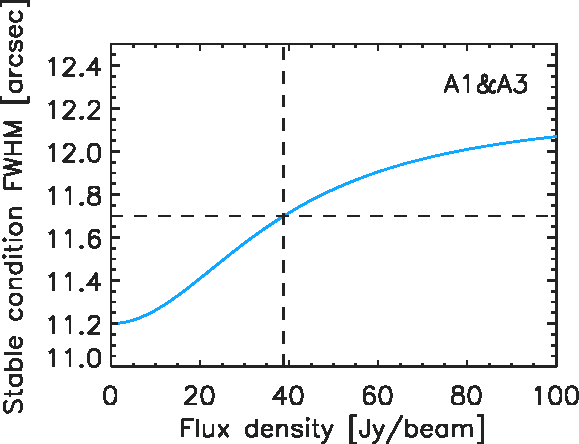
\includegraphics[clip=true, trim={0, -0.3cm, -0.3cm, 0}, width=0.45\textwidth]{Figures/atrier/Photocorr/FWHM_stable_empiric_ref_1mm.pdf}
    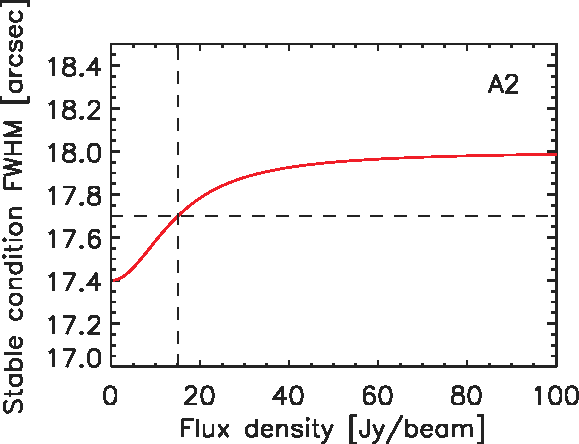
\includegraphics[clip=true, trim={0, -0.3cm, -0.3cm, 0}, width=0.45\textwidth]{Figures/atrier/Photocorr/FWHM_stable_empiric_ref_a2.pdf}
    \caption[Photometric correction pivot Gaussian
      size]{Flux-dependency of the photometric correction pivot
      Guassian size $\sigma_\star$. }
    \label{fig:sigma_stable_vs_flux}
  \end{center}
\end{figure}

In our reference photometric system, as presented in
Sect.~\ref{se:flux_density_equation} and
Sect.~\ref{ap:flux_density_equation},
the flux density is estimated by fitting an amplitude of a fixed-width
Gaussian beam:
%. Using Eqs.~\ref{eq:calfwhm0}, \ref{eq:pointsourcephot}
%and \ref{eq:pointsourcemap}, observed maps are modeled as:
%\begin{equation}
%  M(\theta, \phi) = \frac{A}{2 \pi \sigma_{0}^{2}} e^{-\frac{\theta^{2}}{2\sigma_{0}^{2}}}, 
%\end{equation}
%where $\sigma_{0}$ is the Gaussian beam size corresponding to the
%reference FWHM, which is $12.5''$ for the 1mm arrays and $18.5''$ for
%the 2mm array, as defined in Table~\ref{tab:definitions}.
\begin{equation}
  \hat{S}  = 2 \int \int M(\theta, \phi)\, e^{-\frac{\theta^{2}}{2\sigma_{0}^{2}}} \sin \theta d\theta d\phi.
  \label{eq:flux_density_estimator}
\end{equation}
The beam width $\sigma_{0}$ corresponds to the
reference FWHM, which we recall,  is $12.5''$ for the 1mm arrays and $18.5''$ for
the 2mm array, as defined in Table~\ref{tab:definitions}.

First of all, in stable observing conditions (no beam
broadening effect), the map can be modeled by a single Gaussian of
width $\sigma_\star$ corresponding basically to the main beam size:
\begin{equation}
  M(\theta, \phi) = \frac{A}{2 \pi \sigma_\star^{2}} e^{-\frac{\theta^{2}}{2\sigma_\star^{2}}}.
  \label{eq:pointsource_map}
\end{equation}
Ingesting Eq.~\ref{eq:broader_beam_map} in
Eq.~\ref{eq:flux_density_estimator}, we find that the flux density
estimator depends on the beam size as
\begin{equation}
  \hat{S}  = A \frac{2 \sigma_0^2}{(\sigma_{\star}^2 + \sigma_0^2)}.
\end{equation}
However, the map is calibrated in $FWHM_0$ beam, as described in
Sect.~\ref{se:flux_density_equation}. The absolute calibration factor,
which is evaluating as
$S_{c}(\nu_{0})/\hat{S}_{c}$, has a beam dependency that
compensates the one of the flux density for the source.

On the other hand, if the beam size varies so that the Gaussian part has a size given by
$\sigma'$, the map model rewrites  
\begin{equation}
  M(\theta, \phi) = \frac{A}{2 \pi \sigma'^{2}} e^{-\frac{\theta^{2}}{2\sigma'^{2}}},
  \label{eq:broader_beam_map}
\end{equation}
where the amplitude is the same as in the stable condition case
because the flux density is conserved when integrating over the map. 
The flux density measured using the fixed-width amplitude estimator 
\begin{equation}
  \hat{S'}  = A \frac{2 \sigma_0^2}{(\sigma'^2 + \sigma_0^2)}
\end{equation}
presents a beam-dependency which differs from the one of the primary
calibrator, and which is no longer compensated when performing the
absolute calibration.

To retrieve an unbiased flux density estimate $\hat{S}_{pc}$, the
flux density estimate $\hat{S'}$ has to be corrected as
\begin{equation}
  \hat{S}_{pc} = f(\sigma')\hat{S'},
\end{equation} 
where the photometric correction is 
\begin{equation}
  f(\sigma') = \frac{(\sigma'^2 + \sigma_0^2)}{(\sigma_\star^2+\sigma_0^2)}, 
\end{equation} 
so that $f(\sigma') = 1$ if $\sigma'=\sigma_\star$.

The pivot Gaussian size $\sigma_{\star}$, which corresponds
to the nominal size of the 2D Gaussian fit of the beam that is
measured in stable observing conditions, slightly varies with the
source flux density. Whereas it basically corresponds to the main beam
size for faint to moderately bright point source, it is slightly
larger for sources bright enought for the error beams to be well above
the noise level. In Fig.~\ref{fig:sigma_stable_vs_flux}, we give an
empirical model for the flux dependency of $\sigma_{\star}$: it
smoothly goes from $11.2''$ at 1-mm and $17.4''$ at 2-mm for
moderately bright sources to
$11.7''$ at 1-mm and $17.7''$ at 2-mm at the flux density of Uranus,
then slightly continues increasing for sources brighter than Uranus.


The effect of the \afternoon\ beam size variations, as discussed
in Sect.~\ref{se:beam_variation}, is mitigated by correcting the measured flux
densities using a beam-size dependent function, referred to as the
photometric correction.

In our reference photometric system, as presented in
Sect.~\ref{se:photometric_system}, 
the flux density is estimated by fitting to the data the amplitude of a fixed-width
Gaussian beam:
\begin{equation}
  \hat{S}  = 2 \int \int M(\theta, \phi)\, e^{-\frac{\theta^{2}}{2\sigma_{0}^{2}}} \sin \theta d\theta d\phi.
  \label{eq:flux_density_estimator}
\end{equation}
The beam width $\sigma_{0}$ corresponds to the
reference FWHM, which we recall, is $12.5''$ for the $1\,\rm{mm}$ arrays and $18.5''$ for
the $2\,\rm{mm}$ array, as defined in Table~\ref{tab:definitions}.

First of all, in stable observing conditions (no beam
broadening effect), the observed map of the source can be modeled by a single Gaussian of
width $\sigma_\star$ corresponding basically to the main beam size and
of amplitude $A_\star$:
\begin{equation}
  M(\theta, \phi) = A_\star e^{-\frac{\theta^{2}}{2\sigma_\star^{2}}}.
  \label{eq:pointsource_map}
\end{equation}
Ingesting Eq.~\ref{eq:pointsource_map} in
Eq.~\ref{eq:flux_density_estimator}, we find that the flux density
estimator depends on the beam size as
\begin{equation}
  \hat{S}  = 2\pi \sigma_{\star}^2 \, A_{\star} \, \,  \frac{2 \sigma_0^2}{(\sigma_{\star}^2 + \sigma_0^2)}.
\end{equation}
However, the map is calibrated in FWHM$_0$ beam, as described in
Sect.~\ref{se:photometric_system}. The absolute calibration factor,
which is evaluating as
$S_{c}(\nu_{0})/\hat{S}_{c}$, has a beam dependency that
compensates the one of the flux density for the source.

On the other hand, if the beam size varies so that the Gaussian part has a size given by
$\sigma'$, the map model rewrites  
\begin{equation}
  M(\theta, \phi) = A'\, e^{-\frac{\theta^{2}}{2\sigma'^{2}}}.
  \label{eq:broader_beam_map}
\end{equation}

The flux density measured using the fixed-width amplitude estimator 
\begin{equation}
  \hat{S'}  =2\pi \sigma'^2 \, A' \, \,  \frac{2 \sigma_0^2}{(\sigma'^2 + \sigma_0^2)}
\end{equation}
presents a beam-dependency which differs from the one of the primary
calibrator, and which is no longer compensated when performing the
absolute calibration.

{\lp In addition, because the flux density is conserved when integrating over the map,
the Gaussian amplitudes verify
\begin{equation}
2\pi \sigma_{\star}^2 \, A_{\star} = 2\pi \sigma'^2 \, A'
\label{eq:gaussian_amplitude}
\end{equation}}

To retrieve an unbiased flux density estimate $\hat{S}_{pc}$, the
flux density estimate $\hat{S'}$ has to be corrected as
\begin{equation}
  \hat{S}_{pc} = f(\sigma') \, \hat{S'},
\end{equation} 
where the photometric correction is 
\begin{equation}
  f(\sigma') = \frac{(\sigma'^2 + \sigma_0^2)}{(\sigma_\star^2+\sigma_0^2)}, 
\end{equation} 
so that $f(\sigma') = 1$ if $\sigma'=\sigma_\star$.

% flux-dependency of sigma stable
\begin{figure}[ht!]
  \begin{center}
    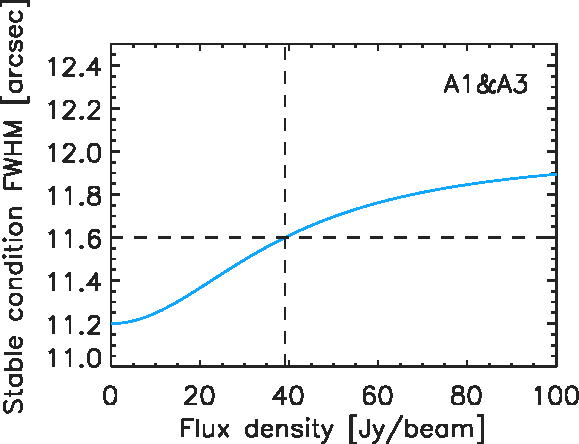
\includegraphics[clip=true, trim={0, -0.3cm, -0.3cm, 0}, width=0.49\linewidth]{Figures/FWHM_stable_empiric_ref_1mm.pdf}
    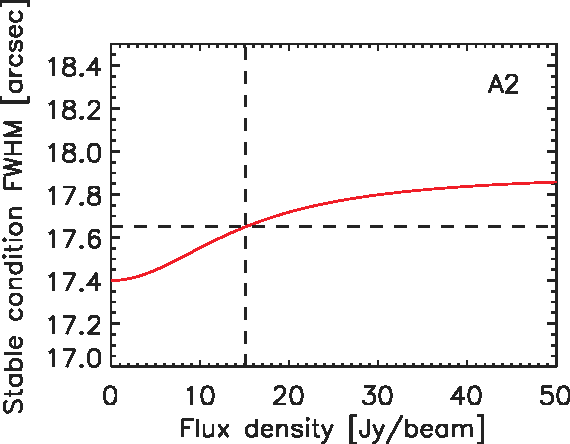
\includegraphics[clip=true, trim={0, -0.3cm, -0.3cm, 0}, width=0.49\linewidth]{Figures/FWHM_stable_empiric_ref_a2.pdf}
    \caption[Photometric correction pivot Gaussian
      size]{Flux-dependency of the pivot size $\sigma_\star$ of the
      Gaussian beam used for the photometric correction. This is measured as the 2D
      Gaussian fit of the map observed in stable conditions.
      The vertical dashed lines correspond to Uranus flux densities in
      the two bands, and the horizontal dashed lines are the
      corresponding measured
      $\sigma_\star$ for Uranus.}
    \label{fig:sigma_stable_vs_flux}
  \end{center}
\end{figure}

As discussed in Sect.~\ref{se:beam_variation}, the beam size is
monitored by fitting a 2D Gaussian of freely varying FWHM.
In practice, the pivot Gaussian size $\sigma_{\star}$ thus corresponds
to the nominal size of the 2D Gaussian fit of the beam that is
measured in stable observing conditions. We find it slightly varies with the
source flux density. Whereas it basically corresponds to the main beam
size for faint to moderately bright point source, it is slightly
larger for sources bright enough for the side lobes to be well above
the noise level. The variation of $\sigma_{\star}$ can be seen as a
correction for fitting the complex beam pattern, as presented in
Sect.~\ref{se:fullbeam}, with a single 2D Gaussian of freely varying
size.

In Fig.~\ref{fig:sigma_stable_vs_flux}, we give an
empirical model for the flux dependency of the FWHM derived from
$\sigma_{\star}$: it
smoothly goes from $11.2''$ at $1\,\rm{mm}$ and $17.4''$ at $2\,\rm{mm}$ for
moderately bright sources to $11.6''$ at $1\,\rm{mm}$ and $17.65''$ at
$2\,\rm{mm}$ at the flux density of Uranus,
then slightly continues increasing for sources brighter than Uranus.
